\documentclass[aps,english,prb,floatfix,amsmath,superscriptaddress,tightenlines,twocolumn,nofootinbib]{revtex4-2}
\usepackage{mathtools, amssymb}
\usepackage{tikz}
\usepackage{tikz-3dplot}
\usetikzlibrary{spy}
\usetikzlibrary{arrows.meta}
\usetikzlibrary{calc}
\usetikzlibrary{decorations.pathreplacing,calligraphy}
\usepackage[utf8]{inputenc}
\usepackage{xcolor}
\usepackage{tcolorbox}

\begin{document}

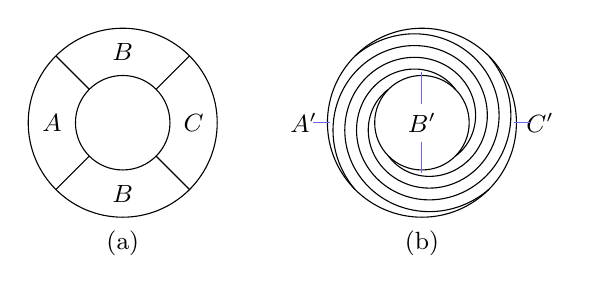
\begin{tikzpicture}
		\begin{scope}[scale=0.6]
			\draw [] (0,0) circle [radius=1];
			\draw [] (0,0) circle [radius=2];
			\draw (45:1) -- (45:2);
			\draw (135:1) -- (135:2);
			
			\draw (-45:1) -- (-45:2);
			\draw (-135:1) -- (-135:2);
			
			\node[] (P) at (0: 1.5)  {\small{$C$}};
			\node[] (P) at (-90: 1.5)  {\small{$B$}};
			\node[] (P) at (90: 1.5)  {\small{$B$}};
			\node[] (P) at (180: 1.5)  {\small{$A$}};
			
			\node[] (P) at (-90: 2.55)  {\small{(a)}};
			
		\end{scope}
		\begin{scope}[xshift=3.8 cm, scale=0.6]
			\draw [] (0,0) circle [radius=1];
			\draw [] (0,0) circle [radius=2];
			\draw [samples=100,smooth,domain=6.28:0,rotate around={45:(0,0)} ] 
			plot ({\x r}:{1+\x/6.28});   
			 
			\draw [samples=100,smooth,domain=6.28:0,rotate around={45+90:(0,0)} ] 
			plot ({\x r}:{1+\x/6.28});   
			
			\draw [samples=100,smooth,domain=6.28:0,rotate around={-45:(0,0)} ] 
			plot ({\x r}:{1+\x/6.28});   
 
			\draw [samples=100,smooth,domain=6.28:0,rotate around={-45-90:(0,0)} ] 
			plot ({\x r}:{1+\x/6.28});
			 
			\node[] (P) at (0: 2.5)  {\small{$C'$}};			 
			\node[] (P) at (90: 0)  {\small{$B'$}};
			\node[] (P) at (180: 2.5)  {\small{$A'$}};
			
		    \node[] (P) at (-90: 2.55)  {\small{(b)}};
			
			\draw [color=blue!60!white] (90:0.4) -- (90:1.07);
			\draw [color=blue!60!white] (-90:0.4) -- (-90:1.07);
			\draw [color=blue!60!white] (0:1.95) -- (0:2.3);
			\draw [color=blue!60!white] (180:1.95) -- (180:2.3);			
		\end{scope}	
	\end{tikzpicture}

\end{document}